\chapter{Исследовательская часть}

В данном разделе будет приведен пример работы программы, а также проведен сравнительный анализ алгоритма поиска для сбалансированного и несбалансированного бинарного дерева поиска.

\section{Демонстрация работы программы}

На рисунке~\ref{img:example}  представлен пример работы программы для поиска в сбалансированном бинарном дереве поиска.
Осуществляется выбор типа дерева поиска, в него происходит добавление элементов, после чего в нём проводится поиск числа.

\begin{figure}[h]
	\centering
	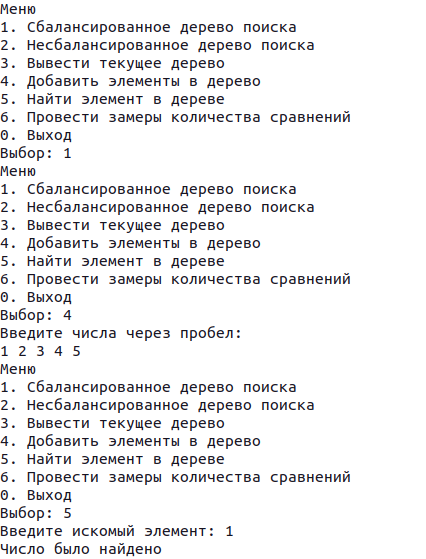
\includegraphics[width=0.5\textwidth]{img/example.png}
	\caption{Пример работы программы}
	\label{img:example}
\end{figure}

\section{Замеры количества сравнений}

Были произведены замеры необходимого количества сравнений для нахождения числа в дереве в худшем и лучшем случае.

Результаты замеров представлены в таблице \ref*{tbl:time}.

\begin{table}[ht]
	\small
	\begin{center}
		\begin{threeparttable}
		\caption{Результаты замеров количества сравнений}
		\label{tbl:time}
		\begin{tabular}{|c|c|c|c|c|}
			\hline
			\multirow{3}{*}{\bfseries Количество узлов} & \multicolumn{4}{c|}{\bfseries Количество сравнений} \\ \cline{2-5}
			 & \multicolumn{2}{c|}{\bfseries АВЛ} & \multicolumn{2}{c|}{\bfseries Несбалансированное} \\ \cline{2-5}
			 & \bfseries Худший & \bfseries Лучший & \bfseries Худший & \bfseries Лучший
			\csvreader{csv/res.csv}{}
			{\\\hline \csvcoli & \csvcolii & \csvcoliii & \csvcoliv & \csvcolv} \\
			\hline
		\end{tabular}
		\end{threeparttable}
	\end{center}
\end{table}

По таблице \ref*{tbl:time} были построены рисунки \ref*{fig:avl-res} -- \ref*{fig:bst-res}, на них можно увидеть зависимость количества сравнений при поиске в худшем случае для АВЛ-дерева и бинарного дерева поиска.

\begin{figure}[h]
	\centering
	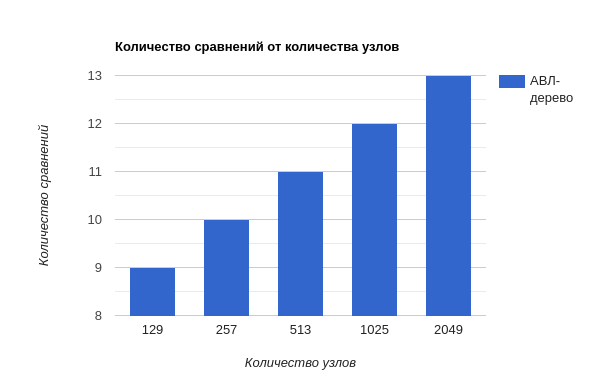
\includegraphics[height=0.4\textheight]{img/avl-graph.png}
	\caption{Результаты замеров количества сравнений в худшем случае при поиске в АВЛ-дереве}
	\label{fig:avl-res}
\end{figure}

\begin{figure}[h]
	\centering
	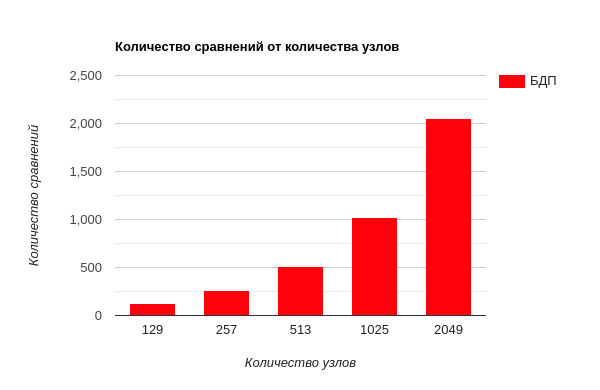
\includegraphics[height=0.4\textheight]{img/bst-graph.png}
	\caption{Результаты замеров количества сравнений в худшем случае при поиске в несбалансированном бинарном дереве поиска}
	\label{fig:bst-res}
\end{figure}

По полученным данным можно увидеть, что количество сравнений при поиске в АВЛ-дереве действительно логарифмически зависит от количества узлов, в то время как для БДП зависимость линейная, что приводит к разнице в 10 и более раз при количестве узлов большем или равном 129.

\section*{Вывод}

В результате эксперимента было получено, что в лучшем случае количество сравнений для АВЛ-дерева и несбалансированного бинарного дерева поиска одинаково и равно 1 для любого рассмотренного количества узлов.
В худшем случае количество сравнений в АВЛ-дереве более чем в 10 раз меньше, чем в несбалансированном бинарном дереве поиска при количестве узлов большем или равном 129.
